\documentclass[a4paper, 14pt]{extarticle}

% Поля
%--------------------------------------
\usepackage{geometry}
\geometry{a4paper,tmargin=2cm,bmargin=2cm,lmargin=3cm,rmargin=1cm}
%--------------------------------------


%Russian-specific packages
%--------------------------------------
\usepackage[T2A]{fontenc}
\usepackage[utf8]{inputenc} 
\usepackage[english, main=russian]{babel}
%--------------------------------------

\usepackage{textcomp}

% Красная строка
%--------------------------------------
\usepackage{indentfirst}               
%--------------------------------------             


%Graphics
%--------------------------------------
\usepackage{graphicx}
\graphicspath{ {./images/} }
\usepackage{wrapfig}
%--------------------------------------

% Полуторный интервал
%--------------------------------------
\linespread{1.3}                    
%--------------------------------------

%Выравнивание и переносы
%--------------------------------------
% Избавляемся от переполнений
\sloppy
% Запрещаем разрыв страницы после первой строки абзаца
\clubpenalty=10000
% Запрещаем разрыв страницы после последней строки абзаца
\widowpenalty=10000
%--------------------------------------

%Списки
\usepackage{enumitem}

%Подписи
\usepackage{caption} 

%Гиперссылки
\usepackage{hyperref}

\hypersetup {
	unicode=true
}

%Рисунки
%--------------------------------------
\DeclareCaptionLabelSeparator*{emdash}{~--- }
\captionsetup[figure]{labelsep=emdash,font=onehalfspacing,position=bottom}
%--------------------------------------

\usepackage{tempora}

%Листинги
%--------------------------------------
\usepackage{listings}
\lstset{
  basicstyle=\ttfamily\footnotesize, 
  %basicstyle=\footnotesize\AnkaCoder,        % the size of the fonts that are used for the code
  breakatwhitespace=false,         % sets if automatic breaks shoulbd only happen at whitespace
  breaklines=true,                 % sets automatic line breaking
  captionpos=t,                    % sets the caption-position to bottom
  inputencoding=utf8,
  frame=single,                    % adds a frame around the code
  keepspaces=true,                 % keeps spaces in text, useful for keeping indentation of code (possibly needs columns=flexible)
  keywordstyle=\bf,       % keyword style
  numbers=left,                    % where to put the line-numbers; possible values are (none, left, right)
  numbersep=5pt,                   % how far the line-numbers are from the code
  xleftmargin=25pt,
  xrightmargin=25pt,
  showspaces=false,                % show spaces everywhere adding particular underscores; it overrides 'showstringspaces'
  showstringspaces=false,          % underline spaces within strings only
  showtabs=false,                  % show tabs within strings adding particular underscores
  stepnumber=1,                    % the step between two line-numbers. If it's 1, each line will be numbered
  tabsize=2,                       % sets default tabsize to 8 spaces
  title=\lstname                   % show the filename of files included with \lstinputlisting; also try caption instead of title
}
%--------------------------------------

%%% Математические пакеты %%%
%--------------------------------------
\usepackage{amsthm,amsfonts,amsmath,amssymb,amscd}  % Математические дополнения от AMS
\usepackage{mathtools}                              % Добавляет окружение multlined
\usepackage[perpage]{footmisc}
%--------------------------------------

%--------------------------------------
%			НАЧАЛО ДОКУМЕНТА
%--------------------------------------

\begin{document}

%--------------------------------------
%			ТИТУЛЬНЫЙ ЛИСТ
%--------------------------------------
\begin{titlepage}
\thispagestyle{empty}
\newpage


%Шапка титульного листа
%--------------------------------------
\vspace*{-60pt}
\hspace{-65pt}
\begin{minipage}{0.3\textwidth}
\hspace*{-20pt}\centering

\includegraphics[width=\textwidth]{emblem}
\end{minipage}
\begin{minipage}{0.67\textwidth}\small \textbf{
\vspace*{-0.7ex}
\hspace*{-6pt}\centerline{Министерство науки и высшего образования Российской Федерации}
\vspace*{-0.7ex}
\centerline{Федеральное государственное бюджетное образовательное учреждение }
\vspace*{-0.7ex}
\centerline{высшего образования}
\vspace*{-0.7ex}
\centerline{<<Московский государственный технический университет}
\vspace*{-0.7ex}
\centerline{имени Н.Э. Баумана}
\vspace*{-0.7ex}
\centerline{(национальный исследовательский университет)>>}
\vspace*{-0.7ex}
\centerline{(МГТУ им. Н.Э. Баумана)}}
\end{minipage}
%--------------------------------------

%Полосы
%--------------------------------------
\vspace{-25pt}
\hspace{-35pt}\rule{\textwidth}{2.3pt}

\vspace*{-20.3pt}
\hspace{-35pt}\rule{\textwidth}{0.4pt}
%--------------------------------------

\vspace{1.5ex}
\hspace{-35pt} \noindent \small ФАКУЛЬТЕТ\hspace{80pt} <<Информатика и системы управления>>

\vspace*{-16pt}
\hspace{47pt}\rule{0.83\textwidth}{0.4pt}

\vspace{0.5ex}
\hspace{-35pt} \noindent \small КАФЕДРА\hspace{50pt} <<Теоретическая информатика и компьютерные технологии>>

\vspace*{-16pt}
\hspace{30pt}\rule{0.866\textwidth}{0.4pt}
  
\vspace{11em}

\begin{center}
\Large {\bf Лабораторная работа № 6} \\ 
\large {\bf по курсу <<Языки и методы программирования>>} \\
\large <<Программа с графическим пользовательским интерфейсом>> \\
\Large Вариант 32
\end{center}\normalsize

\vspace{8em}


\begin{flushright}
  {Студент группы ИУ9-21Б Шиятов Н. \hspace*{15pt}\\ 
  \vspace{2ex}
  Преподаватель Посевин Д. П.\hspace*{15pt}}
\end{flushright}

\bigskip

\vfill
 

\begin{center}
\textsl{Москва 2023}
\end{center}
\end{titlepage}
%--------------------------------------
%		КОНЕЦ ТИТУЛЬНОГО ЛИСТА
%--------------------------------------

\renewcommand{\ttdefault}{pcr}

\setlength{\tabcolsep}{3pt}
\newpage
\setcounter{page}{2}

\section{Задание}\label{Sect::task}

Необходимо разработать на языке Java программу с графическим пользовательским интерфейсом, которая выводит прямоугольник, заданный сторонами a и b, изображённый таким образом, что его длинная сторона составляет угол альфа с осью OX.


\section{Результаты}\label{Sect::res}

Элементы PictureForm.form представлены на рисунке~\ref{fig:form}.

Исходный код программы представлен в листингах~\ref{lst:pictureform}--~\ref{lst:canvaspanel}.

Результат запуска представлен на рисунках~\ref{fig:output1}--~\ref{fig:output2}.


\begin{figure}[!htb]
	\centering
	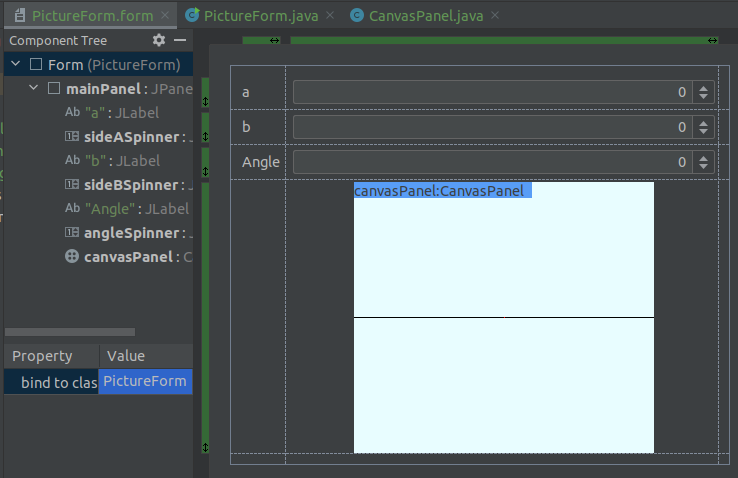
\includegraphics[width=0.8\textwidth]{form.png}
\caption{PictureForm.form}
\label{fig:form}
\end{figure}


\begin{figure}[!htb]
\begin{lstlisting}[language=Java,caption={Класс PictureForm},label={lst:pictureform}]
import javax.swing.*;
import javax.swing.event.ChangeEvent;
import javax.swing.event.ChangeListener;

public class PictureForm {
    private JPanel mainPanel ;
    private JSpinner sideASpinner;
    private JSpinner sideBSpinner;
    private JSpinner angleSpinner;
    private CanvasPanel canvasPanel;

    public PictureForm() {
        sideASpinner.addChangeListener(new ChangeListener() {
            @Override
            public void stateChanged(ChangeEvent e) {
                int a = (int)sideASpinner.getValue();
                canvasPanel.setA(a);
            }
        });
        sideBSpinner.addChangeListener(new ChangeListener() {
            @Override
            public void stateChanged(ChangeEvent e) {
                int b = (int)sideBSpinner.getValue();
                canvasPanel.setB(b);
            }
        });
        angleSpinner.addChangeListener(new ChangeListener() {
            @Override
            public void stateChanged(ChangeEvent e) {
                int alpha = (int)angleSpinner.getValue();
                canvasPanel.setAlpha(alpha);
            }
        });
    }

    public static void main (String[] args) {
        JFrame frame = new JFrame("Rectangle");
        frame.setContentPane (new PictureForm().mainPanel);
        frame.setDefaultCloseOperation(JFrame.EXIT_ON_CLOSE);
        frame.pack();
        frame.setVisible(true);
    }
}
\end{lstlisting}
\end{figure}

\begin{figure}[!htb]
\begin{lstlisting}[language=Java,caption={Класс CanvasPanel},label={lst:canvaspanel}]
import javax.swing.*;
import java.awt.*;
import java.awt.geom.AffineTransform;

public class CanvasPanel extends JPanel {
    private int sideA = 0;
    private int sideB = 0;
    private int angle = 0;

    public void setA(int a) {
        sideA = a;
        repaint();
    }

    public void setB(int b) {
        sideB = b;
        repaint();
    }

    public void setAlpha(int alpha) {
        angle = alpha;
        repaint();
    }

    protected void paintComponent(Graphics g) {
        super.paintComponent(g);

        g.setColor(Color.BLACK);
        g.drawLine(0, getHeight() / 2, getWidth(), getHeight() / 2);

        Graphics2D g2d = (Graphics2D) g;

        int x = getWidth() / 2;
        int y = getHeight() / 2;
        Rectangle shape = new Rectangle(x, y, sideA, sideB);

        AffineTransform tx = new AffineTransform();
        double radians = Math.toRadians(angle);
        tx.rotate(-radians, x, y);
        g2d.setColor(Color.RED);
        Shape newShape = tx.createTransformedShape(shape);

        g2d.draw(newShape);
        g2d.dispose();
    }
}
\end{lstlisting}
\end{figure}

\begin{figure}[!htb]
	\centering
	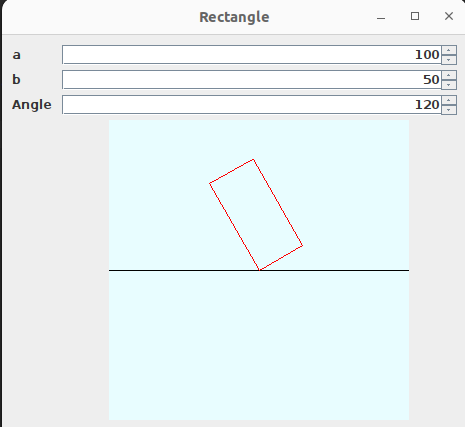
\includegraphics[width=0.6\textwidth]{output1.png}
\caption{Результат}
\label{fig:output1}
\end{figure}

\begin{figure}[!htb]
	\centering
	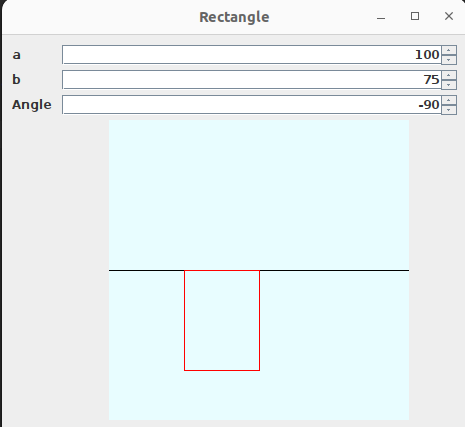
\includegraphics[width=0.6\textwidth]{output2.png}
\caption{Поворот прямоугольника}
\label{fig:output2}
\end{figure}

\end{document}
